%
%     ApJ article: Rapidly Rotating Suns and Active Nests of Convection
%
%     Benjamin Brown
%     JILA and Dept. Astrophysical & Planetary Sciences
%     UCB 440
%     University of Colorado
%     Boulder, CO   803090-0440
%
%     e-mail: bpbrown@solarz.colorado.edu
%
%     Written using using AASTex style sheets
%
%     Submitted April 30, 2008
%     Revision submitted July 1, 2008
%


%*********************************************************************%
%                                                                     %
%              Introduction section                                   %
%                                                                     %
%*********************************************************************%


\chapter{Convection in Rapidly Rotating Younger Suns}
\label{chapter:convection in G1-G10}

%*********************************************************************%
%                                                                     %
%              How our models work section                            %
%                                                                     %
%*********************************************************************%


% now in chapter 2 %

%*********************************************************************%
%                                                                     %
%              Patterns of Convection section                         %
%                                                                     %
%*********************************************************************%



%\section{Convection in Rapidly Rotating Suns}
\label{sec:convection}

We begin our exploration of convection and dynamo action in rapidly
rotating suns with a series of hydrodynamic simulations which sample
rotation rates between $1-10\thinspace\Omega_\odot$.  These correspond
to cases~G1-G10 in Table~\ref{table:sim parameters}.  In these
systems, we explore how the patterns of convection are modified by
more rapid rotation.  We study the resulting differential rotation and
meridional circulation and their scaling with rotation rate.  In
Chapter~\ref{chapter:active nests of convection} we examine how novel
modulated patterns of convection arise in the most rapidly rotating
simulations.  

These two chapters are based on work published in
\citet{Brown_et_al_2008}\footnote{{Brown}, B.~P., {Browning}, M.~K., {Brun}, A.~S., {Miesch}, M.~S., \& {Toomre},
  J., 2008, ``Rapidly Rotating Suns and Active Nests of Convection'', {\sl \apj}, {689},~1354--1372.}
%\footnote{\cite*{Brown_et_al_2008}, 
%``Rapidly Rotating Suns and Active Nests of Convection''} 
and are largely a restatement of that paper.  As the primary author of
this paper, I conducted the simulations presented here, performed the
analysis and wrote the text.  My co-authors provided advice and
guidance throughout the process, helping frame the questions which
form the core of the study.  Preliminary versions of these results
have been presented in \cite{Brown_et_al_2004},
\cite{Brown_SPD_2006}, \cite{Brown_AAS_2007b}, and \cite{Brown_et_al_2007b}.

%%%%%%%%%%%%%%%%%%%%%%%%%%%%%%%%%%%%%%%%%%%%%%%%%%%%%%%%%%%%%%%%%%%%%%%%%%%%%%%%%%%%%%%%%%
\begin{figure}[htbp]
  \begin{center}
    \includegraphics[width=0.7\linewidth]{figs/chapter_3/Figure_2.eps}
  \end{center}
  %\plotone{f2.eps}
  \caption[Convective patterns in mildly turbulent
  simulations]{Convective patterns in mildly turbulent simulations.
  Cases shown are rotating at $(a)$~one, $(b)$~three and $(c)$~five
  times the solar rate.  Shown as snapshots are radial velocities near
  top of layer in global Mollweide projection, with upflows light and
  downflows dark (scaling indicated by accompanying colorbars). Poles are at top and bottom,
  and the equatorial region appears at middle, with equator indicated
  by bold dashed line. Thin dashed lines denote circles of constant
  latitude or longitude, and the thin surrounding line indicates the
  location of the stellar surface at $R_\sol$.  A striking pattern of 
  convection localized into nests near the equator emerges as the
  rotation rate increases. 
  \label{fig:ab2}}
\end{figure}
%%%%%%%%%%%%%%%%%%%%%%%%%%%%%%%%%%%%%%%%%%%%%%%%%%%%%%%%%%%%%%%%%%%%%%%%%%%%%%%%%%%%%%%%%%


\section{Early Results of Modulated Convection}
In our early simulations of rapidly rotating suns we found that
strongly localized states of convection emerged with more rapid
rotation \citep{Brown_et_al_2004}.  A selection of these simulations
in Figure~\ref{fig:ab2} present snapshots of radial velocity near the
top of the domain in global Mollweide projection, showing the entire
spherical surface with minimal distortion.  With more rapid rotation,
a prominent longitudinal modulation appears in the patterns of
equatorial convection.  At the higher rotation rates the equatorial
convection is confined to one or two nests, with streaming zonal flow
filling the regions outside these nests of convection.  These nests
can persist for intervals spanning many hundreds of rotation periods,
often with little change.  Two nest states sometimes evolve into
single nest states as one nest overtakes another.

The simulations shown in Figure~\ref{fig:ab2} are less turbulent than
the cases presented in the rest of this chapter, each possessing
Reynolds numbers that are about three-fold smaller near the surface
than in our new simulations. In these early models, a large portion of
the energy transport in the upper convection zone was carried by
unresolved scales of motion.  This parametrized SGS flux, represented
by $\kappa_0$, dominated transport in the upper 30\% of the convection
zone, leading to weaker enthalpy transport and weaker resolved
convection there.  This parametrized flux acts as a volume cooling term
that removes flux from the regions where it is dominant; the dynamics
were influenced by the presence of this cooling layer.  The cases
presented in detail in this chapter have a narrower unresolved flux layer,
confined now to the upper 10\% of the convection zone, and
consequently much more vigorous convection is realized throughout the
domain.
%
In these more turbulent cases, the phenomena of localized nests of
convection is realized at somewhat higher rotation rates.

%%%%%%%%%%%%%%%%%%%%%%%%%%%%%%%%%%%%%%%%%%%%%%%%%%%%%%%%%%%%%%%%%%%%%%%%%%%%%%%%%%%%%%%%%%
%
%                    ab2_turf full page images
% 
%%%%%%%%%%%%%%%%%%%%%%%%%%%%%%%%%%%%%%%%%%%%%%%%%%%%%%%%%%%%%%%%%%%%%%%%%%%%%%%%%%%%%%%%%%

\begin{figure*}[htbp]
  \begin{center}
    \includegraphics[width=0.9\linewidth]{figs/chapter_3/Figure_3.eps}
  \end{center}
  %\plotone{f3.eps}
  \caption[Convective patterns in primary hydrodynamic cases]
  {Convective patterns in primary hydrodynamic cases.  
    Shown are radial velocity patterns in Mollweide projection at
  $0.95R_\sol$ (left) and differential rotation profiles
  (middle, right) with increasing rotation rate in $(a,e)$
  for~case~G1, $(b,f)$ for~G3, $(c,g)$ for~G5, and
  $(d,h)$ for~G10.  At higher rotation rates the horizontal scale
  of convective cells shrinks at all latitudes and cells are more
  strongly aligned with the rotation axis.  A striking pattern of
  modulated convection emerges at low latitudes with faster rotation,
  consisting of spatially modulated or patchy convection.  These
  active nests of convection are propagating structures which persist
  for long periods of time.  At middle are profiles of mean angular
  velocity $\Omega$ with radius and latitude.  These differential
  rotation profiles all involve fast equators (prograde relative to
  the frame rate $\Omega_0$, indicated by tickmark on scale) and a monotonic decrease of $\Omega$ as
  the poles are approached.  At right are radial cuts of the angular
  velocity at selected latitudes, as labeled.  The dark dashed contour
  denotes the constant propagation rate of the nests where
  discernible. 
  \label{fig:ab2_turf}}
\end{figure*}

%%%%%%%%%%%%%%%%%%%%%%%%%%%%%%%%%%%%%%%%%%%%%%%%%%%%%%%%%%%%%%%%%%%%%%%%%%%%%%%%%%%%%%%%%%



\section{Convective Patterns and Evolution with Rotation}
The variation of convective patterns with increasing rotation rate
$\Omega_0$ in our more rapidly rotating suns
is illustrated in Figure~\ref{fig:ab2_turf}.  Snapshots of the radial velocity near
the top of the domain ($0.95 R_\sol$) are shown in Mollweide
projection for four cases: G1, G3, G5 and G10.
The convection patterns are complex and time dependent, with asymmetries
between the upflows and downflows
owing to the density stratification.  Thus narrow, fast downflow lanes are
surrounded by broad, relatively weak upflows.

There is a clear difference in both the scale and structure of
convection at high and low latitudes.  In the equatorial regions
(roughly $\pm30^\circ$ in latitude), the downflows organize into large
structures (loosely called banana cells) aligned
with the rotation axis, thus extending in the north-south direction.  At high rotation rates this tendency
for alignment becomes pronounced, largely in the spirit of the
Taylor-Proudman theorem, and the downflow network exhibits
little of the east-west branching visible in case~G1.
These downflow lanes propagate in a prograde sense relative
to the bulk rotation rate and do so more rapidly than the differential
rotation which they themselves establish.
%
The nests of convection,
when they appear at the higher rotation rates, propagate at an
intermediate rate as denoted by the heavy dashed contours in
Figure~\ref{fig:ab2_turf}$f-h$.  We defer discussion of the nature of
these nests of convection to Chapter~\ref{chapter:active nests of convection}.
%
Individual convective cells persist for about 10 to 30 days.   
%

In the higher latitude regions, the convection cells are more isotropic and the
downflow network organizes on smaller scales.
Convection in these regions is vigorous and complex, with upflows
and their downflow networks in a constant dance.
The convective cells have a cusped appearance, with downflows leading
upflows as both propagate in a retrograde fashion (most apparent in
Figs~\ref{fig:ab2_turf}$b,c$). 
Strong vortical plumes form in the interstices of the downflow network
at both high and low latitudes.  In the polar regions above the
middle of the convection zone, the sense of
vorticity in these downflow plumes is generally
cyclonic: counterclockwise in the northern
hemisphere and clockwise in the southern.  As they descend through the
mid-layer their vorticity changes and they become largely
anti-cyclonic.  In contrast, the polar upflows are anti-cyclonic
at all depths.   

\clearpage
The latitudinal variation of convection patterns can be in part understood by
considering a cylinder tangent to the base of the convection zone and aligned with
the rotation axis.  Within our geometry, this tangent
cylinder intersects the outer boundary at about $\pm 42^\circ$ of
latitude.  It is well known that in a rotating convective shell the
flow dynamics are different inside and outside of the tangent
cylinder, owing to differences in the connectivity of the flows, the
influence of the Coriolis forces and distance from the rotation axis
\citep[e.g.,][]{Busse_1970}.  These differences become more evident as
the rotation rate, and hence the rotational constraints on the
convection, increases.
With more rapid rotation the longitudinal extent of the convective cells
becomes progressively smaller.
%
%
Linear theory, in the Boussinesq approximation, predicts that the
wavenumber of the most unstable mode scales with rotation as
$m \propto \mathrm{Ta}^{1/6} \propto \Omega_0^{1/3}\nu^{-1/3}$ \citep[e.g.,][]{Chandrasekhar_1961,
  Dormy_et_al_2004} for polar and equatorial convection.  This effect
is found in anelastic systems as well \citep{Glatzmaier&Gilman_1981}
and in our simulations is evident at both high and low latitudes.  

Shown at right in Figures~\ref{fig:ab2_turf}$e-h$ are the
profiles of differential rotation (as angular velocity $\Omega$)
realized in these simulations.  These $\Omega (r,\theta)$ profiles are
azimuthally and temporally averaged over a period of roughly
200~days.  All of our more rapidly rotating stars exhibit
solar-like differential rotation profiles, with prograde (fast)
equators and retrograde (slow) poles.  Contours of constant angular
velocity are aligned nearly on cylinders, influenced by the
Taylor-Proudman theorem, though recent simulations of solar convection
suggest that this is sensitive to the treatment of the bottom
thermal boundary condition \citep{Miesch_et_al_2006}.  
%
As first shown in mean-field models by \cite{Rempel_2005} and then in
global-scale convection models by \cite{Miesch_et_al_2006},
introducing a weak latitudinal gradient of entropy at 
the base of the convection zone, consistent with a thermal wind balance in a
tachocline of shear, can serve to rotate the $\Omega$ contours toward the more
radial alignment deduced from helioseismology without significantly
changing either the overall $\Omega$ contrast with latitude or the
convective patterns.  We expect similar behavior here, as briefly
explored by \cite{Ballot_et_al_2007} in younger suns with deeper
convection zones, but have not
explored this issue in detail at the higher rotation rates.
More rapidly rotating suns may very well also possess tachoclines,
but at this stage there is no observational evidence of this.
Thus we have simplified these simulations by imposing a constant entropy
at the bottom boundary.
%
Our contours of $\Omega$ in Figure~\ref{fig:ab2_turf} 
show some differences between the northern and southern
hemispheres, particularly at higher latitudes, and these differences
decrease with more rapid rotation.  The patterns of convection are not
simply symmetric about the equator, and thus the accompanying mean
zonal flows can be expected to show some variations between the
two hemispheres.  Also shown are radial cuts of $\Omega$ at six fixed
latitudes that make evident the angular velocity contrasts with radius
and latitude achieved in these simulations.  The absolute contrast in
latitude and radius clearly grows with rotation rate, and will be
discussed in \S\ref{sec:global scale flows}.

A most striking result of our simulations is the emergence of
persistent, spatially modulated convection in the equatorial regions
at high rotation rates.  At these low latitudes, convection becomes
modulated in longitude and forms distinct active nests where the convective
vigor is enhanced compared to the regions outside.  The amplitude
of the convective motions and enthalpy transport is larger within
these nests, and indeed at the highest rotation rates,
convection in the equatorial band is confined entirely to the nests.
These nests of convection propagate at a velocity distinct from either
the zonal flow of differential rotation or that of the individual
cells of convection and persist for very long periods of time (more
than 5000~days in case~G5). The nature of these active nests of
spatially localized convection will be explored in detail in
Chapter~\ref{chapter:active nests of convection}.

Weak modulation in longitude is already evident at low rotation rates.
When long time series are considered, we have positively identified
nests of convection in all simulations rotating at 
$\Omega_0 \gtrsim 3~\Omega_\sol$.  As the rotation rate increases, the
modulation level gradually increases; at the highest rotation rates
($\gtrsim 7~\Omega_\sol$) the equatorial convection is almost solely
confined to the nests.  The convection realized in case~G10
(Fig.~\ref{fig:ab2_turf}$d$) is marked by this extreme modulation,
with strong upflows and downflows inside the nest and very little
convection in the surrounding regions.  These most rapidly rotating
cases maintain a strong differential rotation profile, even though the
equatorial convection occupies only a narrow interval in longitude.
The regions outside the nest are filled with fast streaming zonal
flows consistent with the differential rotation.



%%%%%%%%%%%%%%%%%%%%%%%%%%%%%%%%%%%%%%%%%%%%%%%%%%%%%%%%%%%%%%%%%%%%%%%%%%%%%%%%%%%%%%%%%%
\begin{figure}[htbp]  
  \begin{center}
  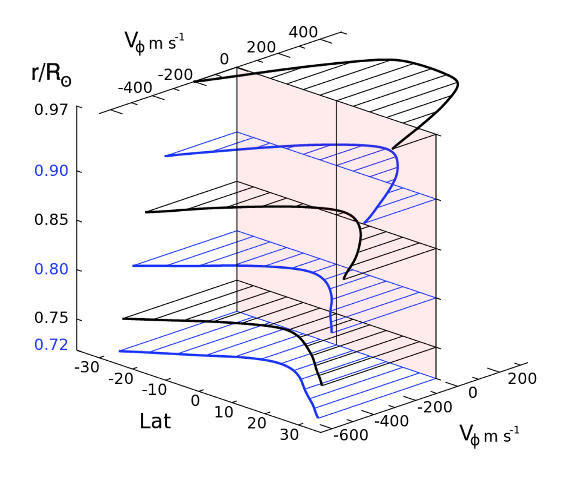
\includegraphics[width=0.75\linewidth]{figs/chapter_3/Figure_4.eps}
  \end{center}
  %\plotone{f4.eps}
  \caption[Profile of $\langle v_\phi \rangle$ in case~G5]
	  {Profile of $\langle v_\phi \rangle$ in case~G5.
	  The variation of mean zonal velocity $\langle v_\phi \rangle$
	  with latitude for case~G5 is sampled at six radial cuts as labeled and
	  shown here relative to the uniform propagation rate of the nests of
	  convection.  The nests experience a strong prograde zonal flow
	  (positive) near the top of layer and a prominent retrograde flow
	  within the lower half.
  \label{fig:G5_patch_shear}}
\end{figure}
%%%%%%%%%%%%%%%%%%%%%%%%%%%%%%%%%%%%%%%%%%%%%%%%%%%%%%%%%%%%%%%%%%%%%%%%%%%%%%%%%%%%%%%%%%


%%%%%%%%%%%%%%%%%%%%%%%%%%%%%%%%%%%%%%%%%%%%%%%%%%%%%%%%%%%%%%%%%%%%%%%%%%%%%%%%%%%%%%%%%%
\begin{figure}[htp]
  \begin{center}
    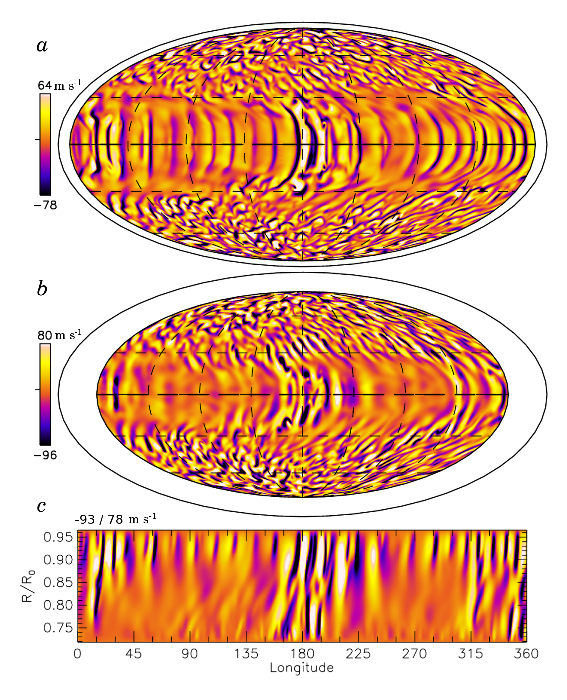
\includegraphics[width=0.8\linewidth]{figs/chapter_3/Figure_5.eps}
  \end{center}
  %\plotone{f5.eps}
  \caption[Connectivity of radial velocity with depth in case~G5]{%
           Connectivity of radial velocity with depth in case~G5.  Shown at
    the same instant in Mollweide view are $v_r$ 
    ($a$)~near top of domain ($0.95R_\sol$), 
    ($b$)~at mid depth ($0.85R_\sol$), 
    and in ($c$)~for an equatorial cut in longitude over full depth range.
    Strong plumes span the convection zone in the equatorial regions
    only within the nest of enhanced convection. The weaker cellular
    flows outside the nests are confined by shear to the upper reaches.
  \label{fig:G5_connectivity}}
\end{figure}
%%%%%%%%%%%%%%%%%%%%%%%%%%%%%%%%%%%%%%%%%%%%%%%%%%%%%%%%%%%%%%%%%%%%%%%%%%%%%%%%%%%%%%%%%%


\subsection{Radial Connectivity of Convection}
The nests of enhanced convection span the
convection zone and propagate everywhere at a constant prograde angular velocity
relative to the bulk rotation rate of the star.  A contour
corresponding to this characteristic propagation rate is overplotted
on the differential rotation profiles in Figures~\ref{fig:ab2_turf}$f-h$
for cases~G3, G5 and~G10.  As is
evident from these profiles, the angular velocity associated with the differential rotation
exceeds that of the propagation rate of the nests near the surface and
is slower than that near the base of the convection zone.  The nests of convection
therefore live within an environment of substantial zonal shear with radius, as is
quantified for case~G5 in Figure~\ref{fig:G5_patch_shear}.  Here the
shearing zonal velocity of differential rotation is plotted in latitude at six radial
depths.  At all depths there is substantial zonal flow through the nests of
convection.  

Other studies of solar convection with ASH show that strong
downflow lanes extend throughout the entire depth of the domain
\citep{Miesch_et_al_2000,Brun&Toomre_2002,Miesch_et_al_2008}.  In our
more rapidly rotating stars, this connectivity with depth changes
markedly, as is illustrated for case~G5 in
Figure~\ref{fig:G5_connectivity} showing radial velocities throughout
the convection zone.  In these rapidly rotating suns, the strong
variation of mean zonal flow with radius in the equatorial regions
prevents all but the strongest downflows from spanning the convection
zone.  Within the nest of enhanced convection the plumes are able to
traverse the convection zone.  Yet in the quieter regions outside, the
weaker downflow plumes are truncated by shear before reaching the
middle of the convection zone.  It is evident
(Fig~\ref{fig:G5_connectivity}$c$) that the amplitude of
convective motions is pronounced at all depths within the nest of active
convection.



The downflowing plumes are influenced by the strong radial shear and
some break into multiple cells with radius even before the full blown
nests of localized convection emerge, as is evident already in our
simulation rotating at twice the solar rate (case~G2).
%
When the downflow networks only span a portion of the convection zone
and experience a limited range of the full density stratification, the
importance of compressible effects decreases.  This has important
consequences for the energetics of the simulations, particularly the
radial kinetic energy flux, as will be addressed in
\S\ref{sec:energies}. In contrast, the downflowing plumes in the polar
regions experience much less shear from either the differential
rotation or the relatively weak meridional circulations and continue
to span the entire convection zone depth.


\subsection{Thermal Structuring}

In these rapidly rotating suns, the turbulent alignment of convection
with the rotation axis leads to a net latitudinal transport of enthalpy, 
yielding a prominent latitudinal gradient of
temperature.  The resulting thermal structuring in case~G5 is shown in
Figure~\ref{fig:G5_thermal_structure}, presenting both the mean
temperature profile and representative temperature fluctuations in a snapshot
near the surface.  In the latter, individual convection cells are
associated with small fluctuations with amplitudes of a
few K.  Downflows are generally cool while upflows are
relatively warmer.  The enhanced enthalpy transport within the active
nests of convection appears as positive temperature fluctuations
in the equatorial region.    

%%%%%%%%%%%%%%%%%%%%%%%%%%%%%%%%%%%%%%%%%%%%%%%%%%%%%%%%%%%%%%%%%%%%%
\begin{figure*}[!t]
  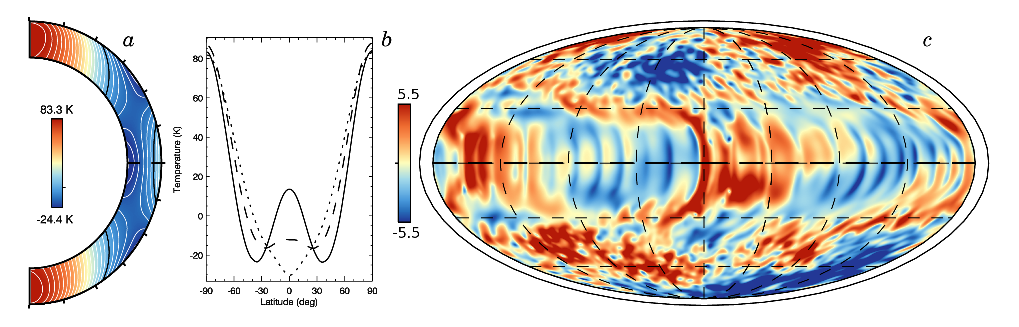
\includegraphics[width=\linewidth]{figs/chapter_3/Figure_6.eps}
  %\plotone{f6.eps}
  \caption[Temperature structures within case~G5]
	  {Temperature structures within case~G5.  Mean latitudinal
  variations in temperature are shown relative to their spherical
  average~$\bar{T}$ in ($a$) as contours with radius and latitude and ($b$) as
  cuts at fixed radii at the top (solid, $0.96R_\sol$), middle
  (dashed, $0.84R_\sol$) and bottom (dotted, $0.72R_\sol$)
  of the domain.  ($c$) Temperature fluctuations in a snapshot near top of
  domain ($0.95R_\sol$) relative to the mean structure in ($a$).
  \label{fig:G5_thermal_structure}}
\end{figure*}
%%%%%%%%%%%%%%%%%%%%%%%%%%%%%%%%%%%%%%%%%%%%%%%%%%%%%%%%%%%%%%%%%%%%%


Evident at high latitudes (Fig.~\ref{fig:G5_thermal_structure}$c$) are
broad spatial structures (in addition to small-scale convection) which
appear in the temperature 
fluctuations and are not readily visible in the maps of radial
velocity (see Fig.~\ref{fig:G5_connectivity} at same instant).
These structures are long lived and appear to be a separate phenomena
from the nests of convection.  The polar patterns propagate in a
retrograde sense more rapidly than the differential rotation in which
they are embedded, and though streaming wakes from the active nests
print weakly into the polar regions, the polar patterns and nests
appear to be distinct phenomena.
The large-scale polar patterns are not evident in the slowly rotating
cases (G1 and G2); in the most rapidly rotating cases this
modulation attains a more complicated form than the two-lobed
structure shown here.

The zonally-averaged thermal structure
(Fig.~\ref{fig:G5_thermal_structure}$a,b$) is quite smooth and is characterized by
warm poles and a cool equator, with yet cooler mid-latitudes.  
In contrast, the mean entropy increases monotonically from
equator to pole, due to effects of pressure.  All of the more rapidly rotating cases
have similar latitudinal thermal profiles, though the temperature
difference between equator and pole increases with more rapid
rotation, as will be discussed further in \S\ref{sec:thermal wind}.
In case~G5, the latitudinal pole to equator temperature contrast is approximately
$100~\mathrm{K}$ throughout the convection zone.  These latitudinal variations remain small
at all rotation rates in comparison to the spherically symmetric
background $\bar{T}$, which ranges from $2.7\times 10^5~\mathrm{K}$ near the surface to
$2.2\times 10^6~\mathrm{K}$ near the bottom of the convection zone (as
shown in Fig.~\ref{fig:ash_structure}).

 

%*********************************************************************%
%                                                                     %
%              Global scale flows section                             %
%                                                                     %
%*********************************************************************%
%\newpage
%\section{Building a Strong Differential Rotation}
%\label{sec:global scale flows}

\section{Thermal Wind Balance}
\label{sec:thermal wind}

Rapidly rotating systems are constrained by the Taylor-Proudman theorem
to have minimal variations in flow dynamics along the direction of the
rotation axis.  In stratified flows, gradients in density and pressure
contribute to baroclinic terms in the vorticity equations
\citep{Pedlosky_1987, Zahn_1992} which maintain flows that can break the
Taylor-Proudman constraint.  In our rapidly rotating suns, convective
plumes tilt toward the rotation axis as rotation effects
increase.  This results in latitudinal as well as radial transport of
enthalpy and builds a latitudinal gradient of temperature and entropy.
Such gradients arise naturally in a rotating convective system even
with uniform thermal boundary conditions.
For a nearly adiabatic stratified, rotating, non-magnetized fluid it
can be shown that in the limit of small Rossby number and negligible
viscous effects the zonal component of the vorticity equations reduces
to the well known thermal wind balance
\citep[e.g.,][]{Brun&Toomre_2002, Miesch_et_al_2006}: 
\begin{equation}
  \frac{\partial \widehat{v_\phi}}{\partial z} = \frac{g}{2 C_P r
  \Omega_0}\frac{\partial \widehat{S}}{\partial \theta} ,
  \label{eqn:TW balance}
\end{equation}
where $z$ is directed along the rotation axis and a hat denotes an
average in longitude and time.  We have further
assumed that the turbulent pressure is negligible.

From equation~(\ref{eqn:TW balance}) it is clear that departures from
rotation constant on cylinders (as observed in the solar interior by
helioseismology) can be maintained by a latitudinal gradient of
entropy.  The left and right hand sides of equation~(\ref{eqn:TW
balance}) are shown for case~G5 in Figure~\ref{fig:TW balance}.  In
the bulk of the convection zone, the differential rotation profiles
realized in these more rapidly rotating suns are substantially in
thermal wind balance.  Significant departures arise near the inner and
outer boundaries (Fig.~\ref{fig:TW balance}$c$) 
where Reynolds stresses and boundary conditions play
a dominant role, as was found in earlier simulations of solar
convection \citep{Brun&Toomre_2002}.

\clearpage


%%%%%%%%%%%%%%%%%%%%%%%%%%%%%%%%%%%%%%%%%%%%%%%%%%%%%%%%%%%%%%%%%%%%%
\begin{figure}[!t]
  \begin{center}
    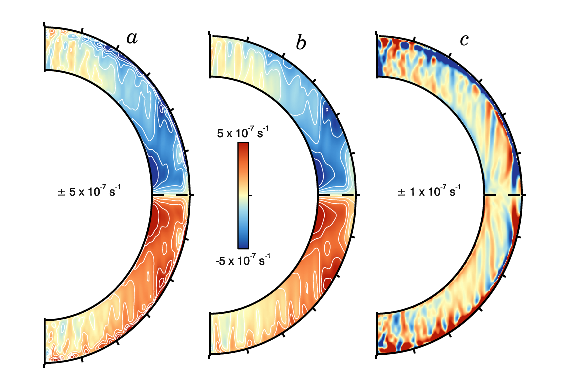
\includegraphics[width=0.7\linewidth]{figs/chapter_3/figure_7.eps}
  \end{center}
  %\plotone{f7.eps}
  \caption[Thermal wind balance achieved in case~G5]{Thermal wind balance achieved in case~G5.  
  $(a)$~Gradients of $\widehat{v_\phi}$ along the rotation axis, $\partial \widehat{v_\phi}/\partial z$,
  $(b)$~the scaled latitudinal entropy gradient from the
  right-hand side of eq.~(\ref{eqn:TW balance}), and $(c)$ their
  difference, with contours in the latter rescaled
  to show the departures near the boundaries.  The bulk of the
  convection zone is in thermal wind balance, but substantial
  departures arise near the top and bottom of the domain where
  Reynolds stresses dominate.
  \label{fig:TW balance}}
\end{figure}
%%%%%%%%%%%%%%%%%%%%%%%%%%%%%%%%%%%%%%%%%%%%%%%%%%%%%%%%%%%%%%%%%%%%%


Another striking property of the thermal wind balance is that
increasing $\Omega_0$ leads to more cylindrical profiles of $\widehat{v_\phi}$
unless $\partial \widehat{S}/\partial \theta$ also adjusts with the rotation
rate.  In our more rapidly rotating suns we find that the latitudinal
gradients of temperature and entropy increase with more rapid
rotation.  The growth of $\Delta \widehat{S}$ (difference between the
surface value of $\widehat{S}$ at say $60^\circ$ and the equator)
with increasing rotation rate $\Omega_0$ is shown in
Figure~\ref{fig:thermal_contrast_with_omega}.  The latitudinal
structure of entropy is always monotonic in these simulations, with
lower entropy at the equator and higher entropy at the poles.
Convection in these more rapidly rotating systems establishes stronger
latitudinal gradients of entropy, but not enough in these simulations to maintain
the $\Omega$ profiles unchanged.


%%%%%%%%%%%%%%%%%%%%%%%%%%%%%%%%%%%%%%%%%%%%%%%%%%%%%%%%%%%%%%%%%%%%%
\begin{figure}[!t]
  \begin{center}
    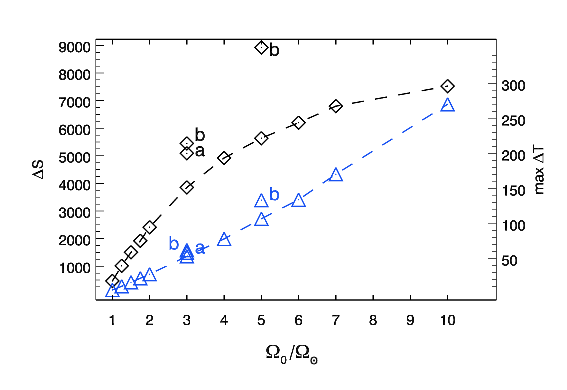
\includegraphics[width=0.7\linewidth]{figs/chapter_3/Figure_8.eps}
  \end{center}
  %\plotone{f8.eps}
  \caption[Scaling of $\Delta \widehat{S}$ and maximal latitudinal
  temperature contrast with $\Omega_0$]{
    Scaling of $\Delta \widehat{S}$ and maximal latitudinal temperature contrast with $\Omega_0$.
    The latitudinal contrast of entropy $\Delta \widehat{S}$  (plotted as diamonds) is measured between equator and
    high latitudes at $0.96R_\sol$.  It increases with more rapid rotation.
    The more turbulent cases (G3a, G3b and G5b as labeled)
    have larger entropy contrasts, in keeping with their generally
    stronger differential rotation.  Blue triangles indicate the
    maximum temperature contrast in latitude at the upper boundary in each simulation.  
  \label{fig:thermal_contrast_with_omega}}
\end{figure}
%%%%%%%%%%%%%%%%%%%%%%%%%%%%%%%%%%%%%%%%%%%%%%%%%%%%%%%%%%%%%%%%%%%%%


Accompanying the growth of $\Delta \widehat{S}$ is a growth in the latitudinal
temperature contrast, as shown by the maximum temperature contrast in
latitude near the stellar surface in
Figure~\ref{fig:thermal_contrast_with_omega}.  Typically, the maximal
contrast occurs between the poles and latitudes of $\pm40^\circ$, as
seen in Figure~\ref{fig:G5_thermal_structure} for case~G5 with a
contrast of about $100~\mathrm{K}$.  In the rapidly rotating
simulations, the primary flux balance in latitude is between thermal
eddy diffusion $\kappa \bar{\rho} \bar{T} \langle \partial S/\partial
\theta \rangle$ and convective enthalpy transport $C_p \bar{\rho}
\langle v_\theta' T' \rangle$.
Here convective transport moves warm
material to the poles as the downflows align more strongly with the
rotation axis while eddy diffusion works to erode the gradient.  
The meridional circulations appear to play a
relatively minor role in maintaining the overall latitudinal entropy
contrast.




\section{Angular Momentum Redistribution}
\label{sec:angular momentum}
In these simulations of stellar convection, complex couplings between
rotation and convection build the profiles of differential rotation and
meridional circulation.
With stress-free boundary conditions at the top and bottom of the
shell there are no net torques and thus the total angular momentum is conserved.
Couplings between rotation and convection lead to a global-scale
redistribution of angular momentum, resulting in the sustained flows of both
differential rotation and meridional circulation.  To assess the
transport of angular momentum in these systems we follow the approach
of \cite{Miesch_et_al_2008}, examining the average radial and latitudinal
angular momentum transport as detailed in their equations~(10)-(12)
\citep[see also][]{Brun&Toomre_2002,Miesch_2005}. 
The angular momentum fluxes from Reynolds stresses (RS), meridional
circulations (MS) and viscous diffusion (VD) are
\begin{eqnarray}
  \vec{F}^{\mathrm{RS}} = \bar{\rho} r \sin{\theta} 
  \left(\langle v_r' v_\phi' \rangle \vec{\hat{r}} +
        \langle v_\theta' v_\phi' \rangle \vec{\hat{\theta}} \right),
	\label{eq:F_RS}\\
%
  \vec{F}^{\mathrm{MC}} = \bar{\rho} {\cal L} 
  \left(\langle v_r \rangle \vec{\hat{r}} +
        \langle v_\theta \rangle \vec{\hat{\theta}} \right),
	\label{eq:F_MC}\\
%
  \vec{F}^{\mathrm{VD}} = -\bar{\rho} \nu r^2 \sin^2{\theta} \nabla \Omega,
  \label{eq:F_VD}
\end{eqnarray}
where 
\begin{equation}
{\cal L} = r \sin\theta \left(\Omega_0 r \sin\theta + \left<v_\phi\right>\right)
\end{equation}
is the specific angular momentum.

%%%%%%%%%%%%%%%%%%%%%%%%%%%%%%%%%%%%%%%%%%%%%%%%%%%%%%%%%%%%%%%%%%%%%
\begin{figure}[htp]
  \begin{center}
    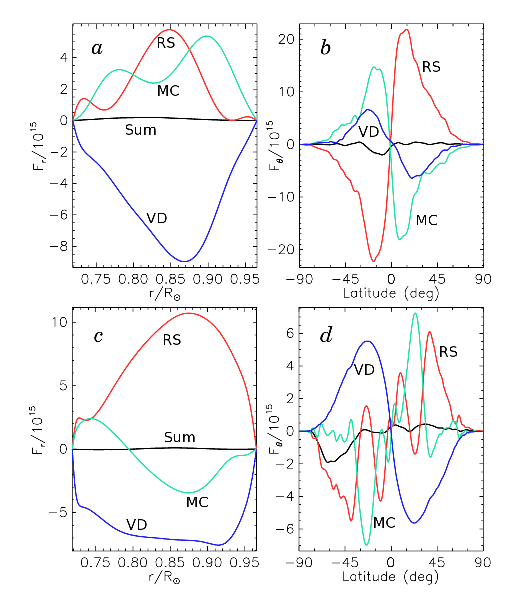
\includegraphics[width=0.7\linewidth]{figs/chapter_3/Figure_9.eps}
  \end{center}
  %\plotone{f9.eps}
  \caption[Angular momentum fluxes in radius and latitude for cases~G1 and G5]
  {Angular momentum fluxes in radius and latitude for cases~G1 and G5.
    Shown are time averages of the integrated radial ($F_r$) and latitudinal ($F_\theta$)
    angular momentum flux for case~G1~($a,b$) and case~G5~($c,d$).
    Contributions arise from Reynolds stresses (RS), meridional
    circulations (MC) and viscous diffusion (VD).  Their total is also
    shown (Sum).  Transport by viscous diffusion remains comparable in all cases,
    while the transport by Reynolds stresses and meridional circulations
    changes markedly with more rapid rotation.
  \label{fig:amom_balance}}
\end{figure}
%%%%%%%%%%%%%%%%%%%%%%%%%%%%%%%%%%%%%%%%%%%%%%%%%%%%%%%%%%%%%%%%%%%%%


The total radial and latitudinal fluxes of angular momentum are shown
for case~G1 and G5 in Figure~\ref{fig:amom_balance}.  Here we have
integrated in co-latitude and radius respectively to deduce the net
fluxes through shells at various radii and through cones at various
latitudes \citep[c.f.,][]{Miesch_2005}.  The three major contributions
arise from Reynolds stresses,  
meridional circulations and viscous terms.  Velocity correlations
lead to net angular momentum transport by Reynolds stresses as
convective structures develop organized tilts and align partially with
the axis of rotation
\citep[e.g.,][]{Brummell_et_al_1998,Brun&Toomre_2002, Miesch_et_al_2008}.  
This alignment is particularly prominent in the fast downflow lanes,
and becomes stronger as rotation increases.



Turning first to our solar case (G1, Fig.~\ref{fig:amom_balance}$a,b$),
we see that in radius the meridional circulations and Reynolds
stresses play similar and nearly equal roles in transporting angular
momentum outward.  The viscous flux meanwhile is negative and
transports angular momentum inward, in keeping with the positive
radial gradient of the differential rotation profile
(eq.~\ref{eq:F_VD}), and the total flux in radius is nearly zero.
The transport in latitude is somewhat different.  Here
meridional circulations combine with viscous fluxes to transport
angular momentum away from the equator and toward the poles
(i.e., positive in the southern hemisphere and negative in the northern
hemisphere). This tendency is opposed by Reynolds stresses, which
continuously accelerate the equatorial regions and dynamically
maintain the angular velocity contrast $\Delta \Omega$ in latitude.

The transport of angular momentum in our more rapidly rotating cases
are all similar in form and are well represented by case~G5
(Fig.~\ref{fig:amom_balance}$c,d$). 
In these more rapidly rotating stars, the radial balance is dominantly
between the Reynolds stresses transporting angular momentum outward and
viscous terms transporting it inward.  The viscous transport is
similar in magnitude to that of case~G1, though the radial boundary
layers are now much narrower.  The transport by Reynolds stresses is nearly twice
as large, and this likely arises from the strong alignment of
convective structures in both polar and equatorial regions. 
In these stars the weaker meridional circulations become relatively
minor and disorganized players in the radial flux balance, moving
angular momentum outward in some regions of the shell and inward in others.
This opposing behavior between the upper and lower convection zone
arises from the meridional circulations breaking into multiple cells
in radius. 

The balances achieved in the latitudinal transport in case~G5
(Fig.~\ref{fig:amom_balance}$d$) are more complex.  As
the rotation rate has increased, the total viscous transport has remained nearly
constant, with the significantly stronger gradients of angular velocity in
the differential rotation profiles
offset by the lower turbulent diffusivities dictated by our path
through parameter space.  That these two opposing actions should
conspire to produce a nearly constant profile of viscous angular
momentum transport is striking and not intuitive.  This is
particularly apparent when we examine the two other terms in the flux balance. 
The meridional circulations have reversed their role from our solar-like case~G1 and
now work with the Reynolds stresses to accelerate the equator and
spin down the polar regions.  The reduced contribution of the meridional
circulations to the total balance arises as the flows become both
weaker and multi-celled in radius and latitude.  
%
The smaller transport by Reynolds stresses appears to result from the
destruction by radial shear of some of the downflow plumes.

\section{Differential Rotation and Scaling with Rotation}
\label{sec:DR}
\label{sec:global scale flows}
In analyzing our simulation results, it is the differential rotation
established by the convection that may yield the most direct contact
with observations.
Stellar observations across the HR diagram indicate that differential
rotation is a common feature in many stars, particularly stars of
spectral class F and later.  In the sun, differential rotation has
been measured throughout the bulk of the convection zone
\citep[as reviewed by][]{Thompson_et_al_2003}, 
but at present for more distant stars only
the surface differential rotation can be inferred.
A variety of observational techniques have been
employed, ranging from photometric variability studies
\citep[e.g.,][]{Donahue_et_al_1996,Walker_et_al_2007}, Doppler imaging
techniques \citep[e.g.,][]{Donati_et_al_2003} and Fourier transform methods
\citep[e.g.,][]{Reiners&Schmitt_2003}.  Typically, these observations seek to measure
the amount of angular velocity contrast at the stellar surface, 
denoted as $\Delta\Omega_*$, though what is being measured may be
somewhat uncertain.  Variations in
$\Delta\Omega_*$ have been found with both rotation rate and spectral
type, however these quantities are correlated and in observations to
date it is difficult to disentangle their possible separate effects 
\citep{Reiners_2006}. 

Different techniques measure fundamentally different tracers of
surface differential rotation, either following variability of
Ca emission (photometric), darkening from inferred starspot presence
(photometric and Doppler imaging) or rotational broadening of absorption lines of
unspotted stars (Fourier transform methods).  Each technique also is most applicable
in only a limited region of stellar parameter space.  As such,
overlapping surveys are in short supply.  Generally,
most observations indicate that the relative
shear, $\Delta\Omega_*/\Omega_*$, depends on the stellar rotation rate
$\Omega_*$ as a power law, though different surveys find different
scalings for the differential rotation, expressed as
\begin{equation}
  \frac{\Delta\Omega_*}{\Omega_*} \propto \Omega_*^n
  \label{eq:relative_contrast}
\end{equation}
(e.g., $n=-0.3\pm0.1$ in \citealt{Donahue_et_al_1996} and 
$n=-0.34\pm 0.26$ in \citealt{Reiners&Schmitt_2003}, but 
$n=-0.85\pm0.10$ in \citealt{Barnes_et_al_2005}). 
Whereas some global models of convection in more rapidly rotating stars have 
been conducted \citep[e.g.,][]{Rudiger_et_al_1998, Kuker&Stix_2001,
  Kuker&Rudiger_2005_A&A, Kuker&Rudiger_2005_AN},
these have been largely carried out in 2-D under the simplifying assumptions
of mean-field theory.

%%%%%%%%%%%%%%%%%%%%%%%%%%%%%%%%%%%%%%%%%%%%%%%%%%%%%%%%%%%%%%%%%%%%%
\begin{figure}[!tb]
  \begin{center}
    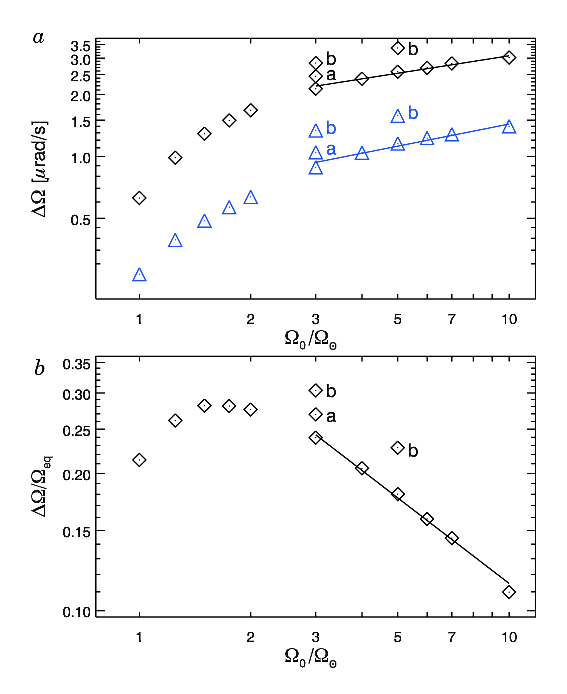
\includegraphics[width=0.7\linewidth]{figs/chapter_3/Figure_10.eps}
  \end{center}
  %\plotone{f10.eps}
  \caption[Scaling of $\Delta \Omega$ and $\Delta
  \Omega/\Omega_{\textrm{eq}}$ with $\Omega_0$]
  {Scaling of $\Delta \Omega$ and $\Delta
  \Omega/\Omega_{\textrm{eq}}$ with $\Omega_0$.
  $(a)$~Angular velocity contrast $\Delta \Omega$ in latitude
  between equator and $60^\circ$ (diamonds)
  and in radius across the shell at the equator (blue triangles). 
  The more rapidly rotating cases appear to follow a power law, which
  for the latitudinal contrast is $m=0.3$ and for the radial contrast
  is $m=0.4$ (as in eq.~\ref{eq:absolute_contrast}).
  %
  $(b)$~Relative latitudinal angular velocity contrast $\Delta
  \Omega/\Omega_{\textrm{eq}}$, with the shown power law having $n=-0.6$
  (as in eq.~\ref{eq:relative_contrast}). 
  The scaling may vary with the path in parameter
  space, as suggested by cases~G3a, G3b~and~G5b.
  \label{fig:ratios_of_omega}}
\end{figure}
%%%%%%%%%%%%%%%%%%%%%%%%%%%%%%%%%%%%%%%%%%%%%%%%%%%%%%%%%%%%%%%%%%%%%


The amount of latitudinal shear observed at the surface $\Delta
\Omega$ is an important quantity both for interpreting stellar
observations and for many 
dynamo theories.  Here we define $\Delta \Omega$ more specifically as the
difference in angular velocity between the equator and say at $60^\circ$
latitude, namely
\begin{equation}
  \Delta \Omega = \Omega_\mathrm{eq} - \Omega_{60} \propto \Omega_0^m.
  \label{eq:absolute_contrast}
\end{equation}
Going to higher latitudes yields comparable behavior.
As shown in Figure~\ref{fig:ratios_of_omega}, we find that
$\Delta \Omega$ increases with rotation rate in our simulations,
with $m=0.3$ in the most rapidly rotating simulations.  The radial shear also
increases with more rapid rotation, and at the equator the difference
between the mean angular velocity at top and bottom of the shell
scales as $m=0.4$ for the rapid rotators.
Because $m<1$, the relative shear $\Delta \Omega / \Omega_\mathrm{eq}$ 
decreases with rotation rate $\Omega_0$ for the rapid rotators, in nearly
a power law fashion for the path through parameter space explored
here.  The scaling exponent from Equation~(\ref{eq:relative_contrast})
exhibited by these cases is $n=-0.6$, but this 
may be influenced by our choice in the scaling of diffusivities with
rotation.  We are 
encouraged that our more turbulent cases~G3b and
G5b, with the same diffusivities at different rotation rates,
exhibit similar behavior.  Our choice of low Prandtl number also has an
effect on this scaling \citep[see ][]{Ballot_et_al_2007}.
Additionally, different treatments of  the SGS unresolved 
flux, which has the most effect in the upper 10\% of the convection
zone, can alter the particular scaling law.  The early simulations
presented in \cite{Brown_et_al_2004} and shown in
Figure~\ref{fig:ab2}, which had a much thicker unresolved flux layer,
had a scaling of $n=-0.8$ in the rapid rotation limit.  We have found
that normalizing $\Delta \Omega$ by $\Omega_0$ rather than
$\Omega_\mathrm{eq}$ leads to a systematic offset for $n$ of about -0.05 in
the inferred scaling law.




\clearpage

\section{Meridional Circulations and Scaling with Rotation}
\label{sec:MC}
The meridional circulations realized within our simulations are of
significance since they can variously transport heat, angular momentum
and even magnetic fields between the equator and the poles, though the
latter are not included in the present simulations.  Our time and
longitude-averaged meridional circulation patterns are shown in
Figure~\ref{fig:MC} for cases~G1, G5 and G10, depicted as streamlines
of mass flux $\Psi$,
\begin{equation}
  r \sin{\theta} \langle \bar{\rho} v_r \rangle = -\frac{1}{r}
  \frac{\partial \Psi}{\partial \theta} 
  \quad \mathrm{and} \quad
  r \sin{\theta} \langle \bar{\rho} v_\theta \rangle = \frac{\partial \Psi}{\partial r}
\end{equation}
and averaged here over a period of at least 150 days.

%%%%%%%%%%%%%%%%%%%%%%%%%%%%%%%%%%%%%%%%%%%%%%%%%%%%%%%%%%%%%%%%%%%%%
\begin{figure}[!htp]
  \begin{center}
    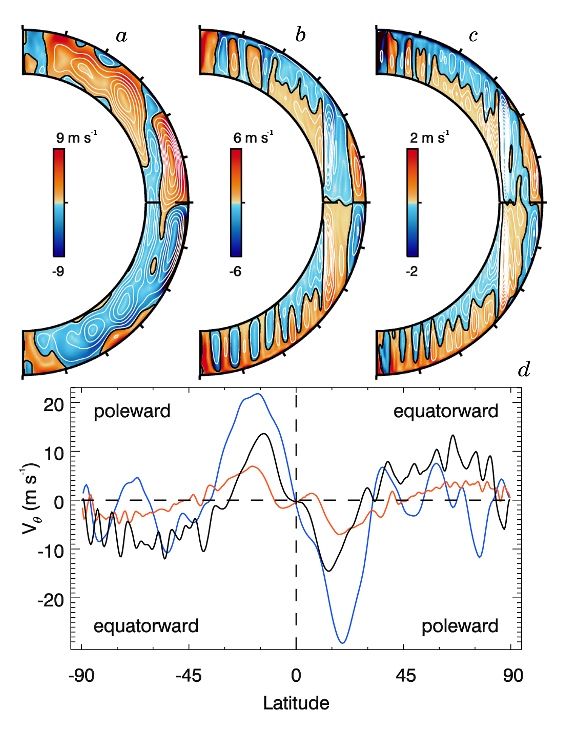
\includegraphics[width=0.7\linewidth]{figs/chapter_3/Figure_11.eps}
  \end{center}
  %\plotone{f11.eps}
  \caption[Changes in structure of meridional circulations with faster rotation]
  {Changes in structure of meridional circulations with faster
  rotation.  Shown are profiles of time and azimuthally averaged 
  meridional circulations with latitude and radius for
  $(a)$~case~G1, $(b)$~case~G5 and $(c)$~case~G10 with
  streamlines of mass flux $\Psi$ overlaid.  Colors indicate the sense
  (red counter-clockwise, blue clockwise) and magnitude of the
  meridional velocity $\langle \vec{v_m} \rangle = \langle v_r \rangle
  \vec{\hat{r}} + \langle v_\theta \rangle \vec{\hat{\theta}}$.  
  With more rapid rotation the meridional
  circulation cells align strongly with the rotation axis and weaken
  in amplitude.  $(d)$ Amplitude of the mean latitudinal component
  $v_\theta$ at the top of the simulation for case~G1~(blue),
  G5~(black), and G10~(red), with regions of poleward
  and equatorward flow denoted.   
  \label{fig:MC}}
\end{figure}
%%%%%%%%%%%%%%%%%%%%%%%%%%%%%%%%%%%%%%%%%%%%%%%%%%%%%%%%%%%%%%%%%%%%%

In our more rapidly rotating cases the meridional circulations have
broken into several cells strongly aligned with the rotation axis
(Fig.~\ref{fig:MC}$b,c$), particularly in the equatorial regions.  Weak
connections between the equatorial and polar regions persist
at the highest rotation rates studied, with organized flows
along the tangent cylinder.  These internal flows weaken with more
rapid rotation.  The meridional circulations are complex and time dependent, with large
fluctuations around the statistically-steady states shown here,
involving variations comparable to or larger than the mean values themselves.  
The circulations are driven by small imbalances between relatively
large forces and their nature is subtle.
The variation of the meridional flows near the surface
($0.96R_\sol$) with rotation rate is shown in Figure~\ref{fig:MC}$d$.  
The amplitude of the
flows decreases substantially with more rapid rotation. Peak
velocities drop from $22~\ms$ in case~G1 to $14~\ms$ in G5 and about $7~\ms$ in G10.  

%As expected from mass conservation, the amplitude of the flows decreases
%strongly with depth.  



The total energy contained in these meridional
circulations decreases quickly with more rapid rotation, as shown in
Figure~\ref{fig:MCKE_vs_omega}.  This drop in energy is independent
of the detailed structure of the convection, showing no change in
behavior at the transition to spatially modulated convection.  In
contrast to the energy contained in convection (CKE) and differential
rotation (DRKE), the energy in the meridional circulations (MCKE) is much
less sensitive to the level of turbulence in any particular
simulation, as indicated by cases~G3, G3a and G3b (detailed in
Table~\ref{table:energy balances}).
The meridional circulations remain important to the global-scale
dynamics as their gradual redistribution of angular momentum
contributes to the large angular velocity gradients in latitude. 
Yet they are inefficient at transporting heat out of the star and at
redistributing thermal material to maintain the latitudinal gradients of
temperature and entropy (which correspond to the thermal-wind component 
of the achieved differential rotation). 

%%%%%%%%%%%%%%%%%%%%%%%%%%%%%%%%%%%%%%%%%%%%%%%%%%%%%%%%%%%%%%%%%%%%%
\begin{figure}[!tp]
  \begin{center}
    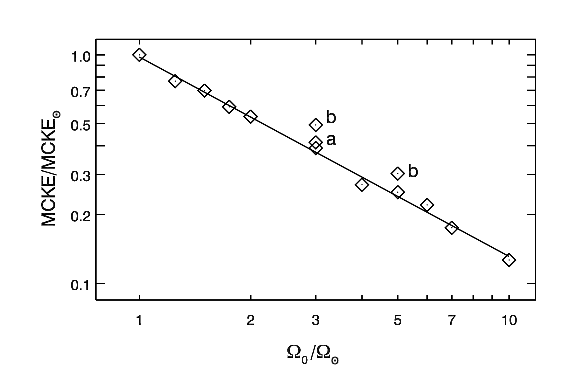
\includegraphics[width=0.7\linewidth]{figs/chapter_3/Figure_12.eps}
  \end{center}
  %\plotone{f12.eps}
  \caption[Scaling of kinetic energy of meridional circulations (MCKE) with $\Omega_0$]
  {Scaling of kinetic energy of meridional circulations (MCKE) with
  $\Omega_0$.  The MCKE is
  normalized by that energy in case~G1 at the solar rate
  ($2.5\times 10^4 \thinspace \mathrm{ergs}~\mathrm{cm}^{-3}$).
  The kinetic energy of these 
  circulations decreases with rotation rate; a power law
  scaling of $\Omega_0^{-0.9}$ is shown for reference.  
   \label{fig:MCKE_vs_omega}}
\end{figure}
%%%%%%%%%%%%%%%%%%%%%%%%%%%%%%%%%%%%%%%%%%%%%%%%%%%%%%%%%%%%%%%%%%%%%

This finding is in striking contrast to the assumptions of many
Babcock-Leighton dynamos, which often take the meridional velocity to
scale as $v_m \propto \Omega$ or $v_m \propto \log{\Omega}$ 
\citep[e.g.,][]{Charbonneau&Saar_2001, Dikpati_et_al_2001}.  
In these models faster meridional circulations lead to shorter dynamo
cycles as surface flux is returned more rapidly to the tachocline.
Currently, the observational data does not appear good enough to
distinguish between the competing models and we will have to await
better measurements of the scaling between cycle period and rotation
rate and possible observations of the meridional circulations
themselves \citep{Rempel_2008}.
Existing 2-D mean-field models of rapidly rotating suns
\citep{Kuker&Stix_2001, Rudiger_et_al_1998, Kuker&Rudiger_2005_A&A}
also predict an increase of meridional circulation velocities with more
rapid rotation.  This is in contrast to their decrease in our simulations.




%*********************************************************************%
\section{Energy Balances and Flux Transport}
\label{sec:energies}

Convection is responsible for transporting the stellar flux emerging
from the deep interior through the convection zone.  In these
simulations, the total luminosity $L(r)$ and its components are
\begin{equation}
  F_e + F_k + F_r + F_u + F_\nu = \frac{L(r)}{4 \pi r^2} = F_t\thinspace,
\end{equation}
with
\begin{eqnarray}
  & F_e = c_p \bar{\rho} \overline{v_r T'}, 
  & F_k = \tfrac{1}{2} \bar{\rho} \overline{v_r v^2}\thinspace,\\
  %
  & F_r = -\kappa_r c_p \bar{\rho} \frac{\mathrm{d} \bar{T}}{\mathrm{d} r}, \quad
  & F_u = -\kappa_0 \bar{\rho} \bar{T} \frac{\mathrm{d}\bar{S}}{\mathrm{d}r}, \quad
    F_\nu = -\overline{\vec{v} \cdot \vec{\scrD}} {\big|}_r\thinspace, \quad ~~
\end{eqnarray}
where $F_e$ is the enthalpy transport by convective motions, $F_k$ is
the kinetic energy flux, $F_r$ is the transport by radiation, $F_u$ is
the unresolved SGS heat flux for parametrized transport by scales of motion below the
resolution of our simulation and $F_\nu$ is the SGS viscous flux.
Figure~\ref{fig:flux_balance} shows the 
flux balance with radius achieved in cases~G1 and
G5, averaged over horizontal surfaces and converted to relative luminosities.   
%
In the deepest layers the radiative flux becomes significant as the
radiative conductivity steadily increases with depth.  By construction
this flux suffices to carry all of the imposed flux through the lower
boundary, where the radial velocities and convective flux vanish.
A similar role is played near the top of the convection zone by the
sub-grid scale transport which yields $F_u$.
The main role of $F_u$ is to transport energy outward through
the impenetrable upper boundary where the convective fluxes vanish and
the remaining fluxes are small, thereby avoiding the 
building of strong superadiabatic radial gradients there. 

The functional form of $\kappa_0(r)$ is chosen so that the entire stellar
luminosity will be transported at the surface of the simulation by $F_u$.
A subtlety of this treatment of the SGS
flux lies in $\mathrm{d} \bar{S}/\mathrm{d}r$.  In the more rapidly
rotating simulations, we find that convection is less able to establish
an adiabatic profile throughout the convection zone.  Instead, much of
the convection zone remains slightly superadiabatic 
($\mathrm{d} \bar{S}/\mathrm{d}r < 0$).  This property is also realized in
local-domain simulations of rapidly rotating convection, where more
rapid rotation leads to enhanced horizontal mixing through vortex
interactions and a resulting decrease in enthalpy transport as
vertical velocities and thermal perturbations become more decorrelated
\citep{Julien_et_al_1996, Brummell_et_al_1996}.  The change of
$\mathrm{d} \bar{S}/\mathrm{d}r$ with rotation rate is shown in
Figure~\ref{fig:ash_structure}$a$ for four of our simulations.  Fixing
the amplitude and structure of $\kappa_0(r)$ across simulations leads
$F_u$ to influence a greater portion of the convection zone at more
rapid rotation, as indicated by the slight growth of $F_u$ in case~G5.
Though this effect becomes stronger as our simulations rotate more
rapidly, at no point in these simulations does $F_u$ transport more
than 10\% of the total luminosity at mid convection zone.  

%%%%%%%%%%%%%%%%%%%%%%%%%%%%%%%%%%%%%%%%%%%%%%%%%%%%%%%%%%%%%%%%%%%%%
\begin{figure}[!ht]
  \begin{center}
    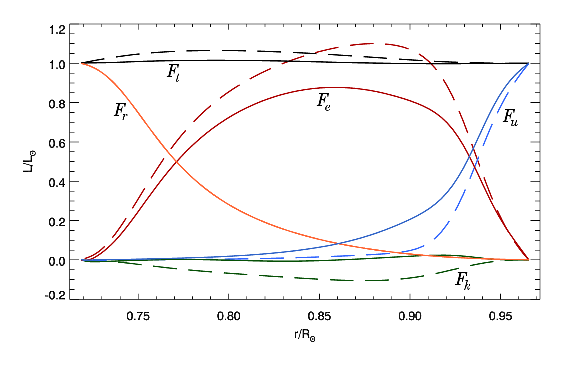
\includegraphics[width=0.7\linewidth]{figs/chapter_3/Figure_13.eps}
  \end{center}
  %\plotone{f13.eps}
  \caption[Average radial energy fluxes in cases~G1 and G5]
  {Average radial energy fluxes in cases~G1 and G5.  Energy fluxes are
  shown with radius with case~G1~(dashed) and G5~(solid) overlain for comparison.
  Shown are the radiative  luminosity ($F_r$), convective enthalpy transport
  ($F_e$), unresolved flux ($F_u$), kinetic energy transport
  ($F_k$), and the total flux through the
  simulation ($F_t$), all normalized by $L_\odot/(4 \pi r^2)$.  
  Case~G1 has a large positive
  convective enthalpy flux throughout the domain, with
  the excess in luminosity largely balanced by an inward flux of kinetic energy.
  At higher rotation rates (as in G5), the kinetic energy flux is nearly zero
  throughout the domain.  In both cases $F_\nu$ is negligible and not shown.
  \label{fig:flux_balance}}
\end{figure}
%%%%%%%%%%%%%%%%%%%%%%%%%%%%%%%%%%%%%%%%%%%%%%%%%%%%%%%%%%%%%%%%%%%%%




In all these simulations, the strong correlations between radial
velocities and temperature fluctuations yield the enthalpy flux $F_e$,
which dominates the energy transport at mid convection zone.  
Both warm upflows and cool downflows serve to transport flux out of
the star, and the two carry comparable amounts of flux to one another
in the rapidly rotating simulations. 
In going to the more rapidly rotating simulations, we find that the
average convective enthalpy flux through the polar regions is greater
than that through the equator.  This is shown in
Table~\ref{table:energy balances}.  In case~G1 (at the solar rate)
slightly more flux is transported through the equator than the poles, but
as the rotation rate increases significantly more flux is transported
through the poles than the equator.  This latitudinal variation
becomes somewhat weaker in our more turbulent cases (G3a, G3b and
G5b), but remains present.  Interestingly, cases G7 and G10 follow
similar trends in their equatorial enthalpy transport, despite the
emergence of strong nests of convection at the equator and the
suppression of convection in the rest of that region.



%%%%%%%%%%%%%%%%%%%%%%%%%%%%%%%%%%%%%%%%%%%%%%%%%%%%%%%%%%%%%%%%%%%%%
%
%     April 26, 2007:
%     These table values are averaged over ~100 days, produced by
%     scalar_study.pro, as called by map_parameter_space.pro 
%
%     Updated   2/26/08 to reflect enthalpy transport from convection alone.
%     Finalized 4/26/08.  That's a wild set of dates.
%
%%%%

\begin{deluxetable}{lcccccccc}
%\begin{deluxetable*}{lcccccccc}
\tablecaption{Flux Balances and Energies\label{table:energy balances}}
\tablewidth{0pt}  % `natural' size
\tablehead{\colhead{Case} 
& \colhead{$F_{e,\mathrm{pole}}$\tablenotemark{a}}
& \colhead{$F_{e,\mathrm{eq}}$\tablenotemark{a}}
& \colhead{$F_{k,\mathrm{pole}}$\tablenotemark{a}}
& \colhead{$F_{k,\mathrm{eq}}$\tablenotemark{a}}
& \colhead{CKE\tablenotemark{b}}
& \colhead{DRKE\tablenotemark{b}}
& \colhead{MCKE\tablenotemark{b}}
& \colhead{$\Delta T_\mathrm{max}$\tablenotemark{c}}
}
\startdata
G1  & 1.014 & 1.140 & -0.118 & -0.190
    &$3.28$  & $2.26$  & $0.025$ & 5.50 \\   
G2  & 1.300 & 0.684 & -0.088 & \phn0.046
    &$2.64$  & $13.2$  & $0.015$ & 28.0 \\  
G3  & 1.349 & 0.628 & -0.077 & \phn0.071
    &$2.40$  & $20.5$  & $0.011$ & 53.5 \\
G4  & 1.327 & 0.631 & -0.065 & \phn0.073
    &$2.21$  & $25.5$  & $0.009$ & 78.5 \\ 
G5  & 1.329 & 0.625 & -0.079 & \phn0.078
    &$2.11$  & $30.1$  & $0.007$ & 107  \\ 
G7  & 1.298 & 0.581 & -0.097 & \phn0.080
    &$1.69$  & $38.7$  & $0.005$ & 171  \\ 
G10 & 1.236 & 0.623 & -0.093 & \phn0.090
    &$1.51$  & $47.1$  & $0.003$ & 271  \\[0.25cm]  

G3a & 1.268 & 0.655 & -0.071 & \phn0.068
    &$2.73$  & $27.7$  & $0.012$ & 58.7 \\  
G3b & 1.101 & 0.780 & -0.065 & \phn0.043
    &$3.34$  & $37.9$  & $0.013$ & 62.4 \\  
G5b & 1.172 & 0.668 & -0.047 & \phn0.081 
    &$2.44$  & $57.4$  & $0.008$ & 134  \\[0.1cm]
\enddata
\tablenotetext{a}{Average convective enthalpy ($F_e$) and kinetic
  energy ($F_k$) fluxes at mid-layer scaled by the solar
  flux, shown for polar (latitudes above $\pm 60^\circ$) and
    equatorial (from $\pm 30^\circ$) regions.}
\tablenotetext{b}{Kinetic energy density relative to
  the rotating coordinate system, for
  convection (CKE), differential rotation (DRKE) and meridional
  circulations (MCKE), averaged over the full shell and over $\sim$ 300 days; units
     are $10^6~\mathrm{erg}\thinspace \mathrm{cm}^{-3}$.}
\tablenotetext{c}{Maximum temperature contrast at $0.96 R_\sol$ in K, typically
  occurring between pole and~$\pm40^\circ$}
%\end{deluxetable*}
\end{deluxetable}
%%%%%%%%%%%%%%%%%%%%%%%%%%%%%%%%%%%%%%%%%%%%%%%%%%%%%%%%%%%%%%%%%%%%%

In case~G1, convection transports slightly more enthalpy than
the solar luminosity.  This over luminosity is balanced by an inward
transport of kinetic energy, which is primarily due to compressible
effects and the transport of $v_r^2$ within strong downflows
that span the convection zone and feel the full density
stratification \citep{Hurlburt_et_al_1986}.  
In the more rapidly rotating cases, the prominent differential rotation
shears apart the convection cells.  The downflows
lose much of their coherence and only the strongest downflows within
the nests of localized convection survive to span the full
convection zone.  Individual downflows thus feel less density
stratification, and compressible effects become less important, leading
to a balance in the transport of $v_r^2$ between the upflows and
downflows.  Instead, as shown in Table~\ref{table:energy balances} the
sense of $F_k$ reverses in the equatorial regions,
becoming dominated by the outward transport of $v_\phi^2$.  The polar
regions remain largely unchanged and the total $F_k$ across spherical surfaces
is nearly zero.


Volume-averaged energy densities for a selection of our simulations
are shown in Table~\ref{table:energy balances}.  At the solar rotation
rate, convective kinetic energy (with kernel
$\frac{1}{2}\bar{\rho}v^{'2}$ and labeled CKE) and the kinetic energy in the
average differential rotation 
($\frac{1}{2}\bar{\rho}\langle v_\phi \rangle^2$, DRKE) are comparable.  As the
rotation rate is increased, DRKE grows strongly and convective energy
decreases slightly, leading DRKE to dominate the total energy budget.
This is true even in our significantly more turbulent solutions.  
The energy in meridional circulations ($\frac{1}{2}\bar{\rho}(\langle
v_r \rangle^2 + \langle v_\theta \rangle^2)$, MCKE) is always small,
and decreases in both magnitude and percentage of the total energy
with more rapid rotation. 



\section{Conclusions}
\label{sec:convection conclusion}

When stars like our sun are young they rotate much more rapidly than
the present sun.  In these stars rotation must strongly
influence the convective motions and may lead to stronger global-scale
dynamo action. In this chapter, we have explored the effects of more rapid
rotation on global-scale convection in simulations of stars like our
sun.  The mean zonal flows of  differential rotation become much
stronger with more rapid rotation, scaling as $\Delta \Omega \propto \Omega_0^{0.3}$ or as
$\Delta \Omega/\Omega_\mathrm{eq} \propto \Omega_0^{-0.6}$.  In striking
contrast, the meridional circulations become much weaker with more
rapid rotation, and the energy contained in them drops approximately
as $\Omega_0^{-0.9}$.  Accompanying the growing differential rotation
is a significant latitudinal temperature contrast, with amplitudes of
$100~\mathrm{K}$ or higher in the most rapidly rotating cases.  The maximum
temperature contrast near the surface occurs between the hot poles and
the cool mid latitudes at about $\pm 40^\circ$.  If this latitudinal
temperature contrast prints through the vigorous convection at the
stellar surface, it may appear as an observable latitudinal variation
in intensity.  The thermal contrast would presumably persist for long
periods compared to stellar activity, offering a way to disentangle
this intensity signature from that caused by spots of magnetism at the
stellar poles.

\clearpage
These simulations are entirely hydrodynamic and this provides a major
caveat to our findings on the scaling of differential rotation 
and latitudinal temperature contrast with rotation rate $\Omega_0$.
Prior MHD simulations of stellar convection have demonstrated that in
some parameter regimes strong dynamo-generated magnetic fields can
react back strongly on the differential rotation, acting to lessen
angular velocity contrasts or largely eliminate them
\citep[e.g.,][]{Brun_et_al_2005, Featherstone_et_al_2007,Browning_2008}.  
It is unclear whether the scaling trends identified here for
differential rotation as a function of $\Omega_0$ will survive in the
presence of dynamo action and magnetic fields.  Likewise, magnetic
fields may lessen the strong temperature contrasts realized here,
doing so through their feedback on the convective flows and energy transport.
We expect that the weaker meridional circulations may be less affected
by magnetic feedbacks, and thus the prediction that meridional
circulations lessen in energy and amplitude with more rapid rotation
may be of greater significance though harder to confirm
observationally.  Weaker meridional circulations in more rapidly
rotating stars will have a strong impact on many theories of stellar
dynamo action, including the Babcock-Leighton flux-transport model favored for
solar-type stars.   To answer such questions, we will turn in due
course in Chapters~\ref{chapter:case D3}-\ref{chapter:menagerie of dynamos} 
to MHD simulations that capture dynamo action in the bulk of the convection zone.  

%The
%parameter space 
%We have begun simulations to explore the dynamo action realized at
%various rotation rates, and its impact upon the flows described here.
%Preliminary results appear in \cite{Brown_et_al_2007c} and more
%detailed results will be forthcoming shortly.


